\documentclass[article,A4,12pt]{llncs}
\usepackage[T1]{fontenc}
\usepackage{amsmath}
\usepackage{amssymb}
\usepackage{amsfonts}
\usepackage{mathrsfs, bm}

\usepackage{graphicx}
\usepackage{tabularx}
\usepackage{subfig}
\usepackage{epsf,times}
\usepackage{color}
\usepackage{wrapfig}
\usepackage{cases}
\usepackage{multicol}

\usepackage[T1]{fontenc}
%\newcommand{\tmname}[1]{\textsc{#1}}
%\newcommand{\tmop}[1]{\ensuremath{\operatorname{#1}}}
%\newcommand{\tmsamp}[1]{\textsf{#1}}
%\newcommand{\tmtextsc}[1]{{\scshape{#1}}}
%\newcommand{\tmtextsl}[1]{{\slshape{#1}}}
%\newcommand{\tmtexttt}[1]{{\ttfamily{#1}}}

\leftmargin=0.0cm
\oddsidemargin=0.5cm
\evensidemargin=0.5cm
\topmargin=0cm
\textwidth=16.0cm
%\textheight=21.5cm
\textheight=20.0cm
\pagestyle{plain}
\setlength{\columnsep}{20pt}

\def\m{\mathbf{m}}
\def\H{\mathbf{H}}
\def\E{\mathbf{E}}
\newcommand{\vepsi}{{\varepsilon}}
\def\hnorm#1#2{\vert\,#1\,\vert_{#2}}
\newcommand{\R}{{\mathbb R}}
\newcommand{\Sph}{{\mathbb S}}
\def\x{\mathbf{x}}
\def\hvec{\overline{\mathbf{h}}}
\def\evec{\overline{\mathbf{e}}}

\newcommand{ \etal}{\mbox{\emph{et al. }}}

\newcommand\vect[1]{\mbf{#1}}
\newcommand{\mbf}[1]{\mbox{\boldmath$#1$}} 
\newcommand{\RC}[1]{#1 $\times$ #1 $\times$ #1}
\def\um{$\mu$m}
\def\C{$^{\circ}\mathrm{C}$}

\newcommand{\Rmnum}[1]{\expandafter\@slowromancap\romannumeral #1@}

% DEFINITION OF CUSTOM FONT SIZE
\newcommand{\customfontA}{\fontsize{50}{55}\selectfont}
\newcommand{\customfontB}{\fontsize{14.4}{20}\selectfont}
\newcommand{\customfontC}{\fontsize{30}{35}\selectfont}

\DeclareMathAlphabet{\mathpzc}{OT1}{pzc}{m}{it}

\def\clovek#1{\noindent\bgroup\vbox{\noindent#1}\egroup\vskip1em}

% TO INPUT BACKGROUND IMAGE
\usepackage{eso-pic}
\newcommand\BackgroundPic{
\put(0,0){
\parbox[b][\paperheight]{\paperwidth}{
\vfill
\centering
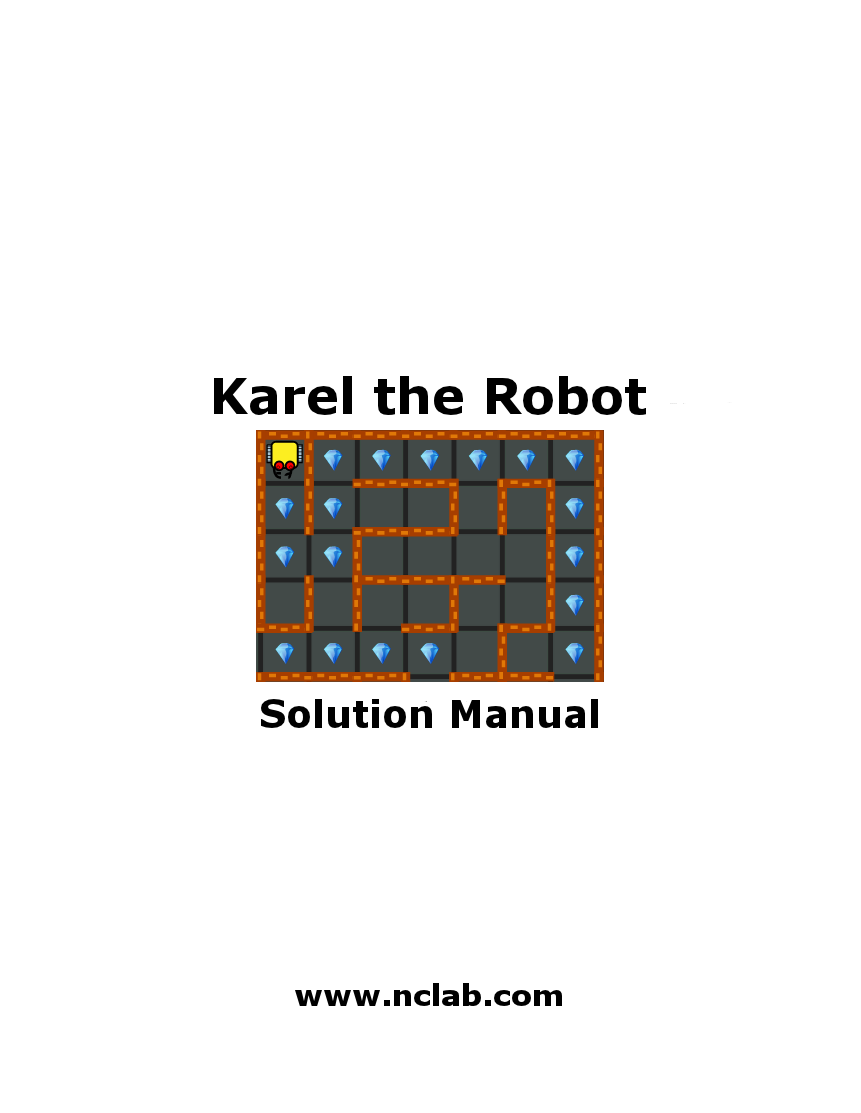
\includegraphics[width=\paperwidth,height=\paperheight]{img/karel-sol-frontpage.png}
%\includegraphics[width=\paperwidth,height=\paperheight]{img/background.jpg}
\vfill
}}}

\begin{document}

% INPUTTING BACKGROUND IMAGE
\AddToShipoutPicture{\BackgroundPic}
\vbox{}
\pagestyle{empty}
\newpage
\textwidth=15.5cm
\ClearShipoutPicture
\newpage

%%%%%%%%%%%%%%%%%%%%%%%%%%%%%%%%%%%%%%%%%%%%%%%%%%%%%%%%%%%%%%%%%%%%%%%%%

\section*{}
\small
\subsection*{About NCLab}
Networked Computing Laboratory (NCLab) is a popular Internet-based framework for 
programming, mathematics, computer modeling, 
and scientific computing. It serves students, instructors, researchers, and the general 
public. NCLab can be used free of charge for personal non-commercial purposes such as 
private hobby or self-education, as well as for individual non-funded academic research.
All other use is subject to {\bf purchasing a license} for a symbolic fee. The fees are as low as 
\$1 per user per month for educational use, and they are used to support the development 
and operational expenses. NCLab is a product of FEMhub Inc. The name "NCLab" is 
registered with the U.S. Patent and Trademark Office (USPTO) under Trademark No. 85420518.

\subsection*{Terms of Use and Pricing}
More details on purchasing a license and using NCLab are provided in the online documents 
{\bf Pricing} and {\bf Terms of Use} that are accessible from NCLab's home page 
{\tt http://nclab.com}.

\subsection*{Contact Information}
General inquiries: {\tt info@femhub.com}\\
Sales: {\tt sales@femhub.com}\\
NCLab support: {\tt support@nclab.com}\\
Agros \& Hermes support: {\tt support@femhub.com}\\
Web page: {\tt http://femhub.com}\\
{Physical address}\\
FEMhub Inc.\\
5490 Twin Creeks Dr.\\
Reno, NV 89523

\subsection*{About This Publication}
This publication can be copied and distributed without any restrictions
as long as reference to NCLab and FEMhub Inc. is preserved.

\subsection*{NCLab's Karel vs. the Original Version}
This publication features {\em Karel the Robot}, a programming language 
designed by Richard E. Pattis. Compared to its original version that was
strongly influenced by Pascal, the NCLab version is closer to Python.
There are some other differences as well that make Karel in NCLab easier to use 
for kids -- Karel collects gems instead of beepers, he has a home in the 
maze, and he uses commands that are much easier for kids to understand
and type. For example, {\tt pickbeeper} was replaced with {\tt get}, 
{\tt front-is-clear} was replaced with {\tt wall}, etc. Even the Python 
colons following every command are omitted because using the SHIFT key 
was causing difficulties to some 5 years old programmers. 
Otherwise we have not changed Pattis' original ideas and all functionality 
covered in Pattis' book is available in the Basic Version of the Programming
module free of charge. 

\normalsize

\newpage
%{\ }
\setcounter{tocdepth}{2}
\tableofcontents
%\pagestyle{plain}

\newpage

\pagestyle{plain}
\setcounter{page}{1}

%%%%%%%%%%%%%%%%%%%%%%%%%%%%%%%%%%%%%%%%%%%%%%%%%%%%%%%%%%%%%%%%%%%%%%%%%

\section{Solutions to Tutorial Games}

This Solution Manual provides sample solutions to all games in the 
Programming mode of the tutorial "First Course in Programming with
Karel the Robot", as well as to some other games.

\subsection{B01 - Go Command}
\begin{verbatim}
go
go
\end{verbatim}

\subsection{B02 - Get Command}
\begin{verbatim}
go
get
go
get
go
get 
go
\end{verbatim}



\subsection{B03 - Turn Command}
\begin{verbatim}
turn 
go
turn
go
get
turn
turn
turn
go
turn 
go
\end{verbatim}



\subsection{B04 - Put Command}
\begin{verbatim}
go
get
turn
turn
go
go
put
turn
turn
go
turn 
go
\end{verbatim}


\subsection{C01 - Ten Steps}
\begin{verbatim}
repeat 10
  go
\end{verbatim}



\subsection{C02 - Nine Gems}
\begin{verbatim}
repeat 10
  go
  get
\end{verbatim}




\subsection{C03 - Diamond Staircase}
\begin{verbatim}
repeat 10
  turn
  go
  repeat 3
    turn
  go 
  get
\end{verbatim}



\subsection{C04 - Nesting}
\begin{verbatim}
repeat 4
  repeat 7
    go
    get
  turn
\end{verbatim}


\subsection{D01 - Foggy Road}
\begin{verbatim}
repeat 10
  go
  if gem
    get
\end{verbatim}



\subsection{D02 - Secret Chest}
\begin{verbatim}
repeat 11
  go
  turn
  go
  if not gem
    put
  repeat 2
    turn
  go
  turn
\end{verbatim}


\subsection{E01 - Looking for Home}
\begin{verbatim}
while not home
  go
\end{verbatim}




\subsection{E02 - Hide-and-Seek}
\begin{verbatim}
while not home
  go
  if gem
    turn
    get
\end{verbatim}






\subsection{F01 - Swirling Tornado is Back}
\begin{verbatim}
def right_turn
  repeat 3
    turn

def four_steps
  repeat 4
    go

def walk_edge
  right_turn
  four_steps
  get
  
# Main program.
while not home
  walk_edge
\end{verbatim}




\subsection{F02 - Diamond Staircase is Back}
\begin{verbatim}
# Definition of the new command
# "turn_right". This should be 
# your last step, after having 
# defined "one_step".
def turn_right
  repeat 3
    turn

# Definition of the new command
# "one_step". This whould be done
# after the main program is written.
def one_step
  turn
  go 
  turn_right
  go
  get

# Main program, this should be 
# your first thing to write.
while not home
  one_step
\end{verbatim}



\subsection{F03 - Pirate Ship}
\begin{verbatim}
# The three commands below are 
# elementary and you should be
# defining them as the last thing.
# Read this code from below. 
# Long step.
def long_step
  repeat 2
    go

# Turn back.
def turn_back
  repeat 2
    turn

# Right turn.
def turn_right
  repeat 3
    turn

# Get pair of gems that lie across 
# the aisle, and move to next pair.
# This should be your third part
# of code to write.
def get_two
  go
  turn
  go
  get
  turn_back
  long_step
  get
  turn_back
  go
  turn_right


# Empty an entire aisle and 
# get ready for the next one.
# This should be your second 
# part of the code to write.
def empty_aisle
  go
  turn_right
  while not wall
    get_two
  turn_back
  while not wall
    go
  turn_right
  long_step
    
# Karel does not know how many 
# aisles there are, so he will 
# be emptying them until he 
# gets home. This should be your
# first part of code to write.
while not home
  empty_aisle
\end{verbatim}



\section{Solutions to Selected Additional Games}



\subsection{Easy - Easy Pick}
\begin{verbatim}
while not home
  if gem 
    get
  go
\end{verbatim}




\subsection{Easy - Gem Jam!}
\begin{verbatim}
while not home
    while not wall
        if gem 
          get
        go
    turn
\end{verbatim}





\subsection{Intermediate - Four Star Hotel}
\begin{verbatim}
def right_turn
  repeat 3 
    turn
  
def go_get_go
  go
  get
  go

def get_star
  repeat 2
    go
  repeat 4
    go_get_go
    turn
  go
  turn
  go_get_go

repeat 3
  get_star
  go
  right_turn
get_star
right_turn
repeat 3
  go
\end{verbatim}





\subsection{Intermediate - The Matrix (Solution 1)}
\begin{verbatim}
# Right turn.
def turn_right
  repeat 3
    turn

# Go forward till you reach wall,
# collect gems on the way.
def get_till_wall
  while not wall
    go
    if gem
      get
  
def there_and_back:
  repeat 2
    go
  turn_right
  get_till_wall
  turn
  go
  if gem
    get
  go
  if gem
    get
  turn
  get_till_wall
  turn_right
  
repeat 4
  get_till_wall
  turn_right
  
repeat 3
  there_and_back  
  
go
go
turn_right

repeat 2
  there_and_back  

repeat 2
  turn
while not wall
  go
turn
while not home
  go
\end{verbatim}

\subsection{Intermediate - The Matrix (Solution 2)}
\begin{verbatim}
# Right turn.
def turn_right
  repeat 3
    turn

# Go forward till you reach wall,
# collect gems on the way.
def get_till_wall
  while not wall
    if gem
      get
    go
    if gem
      get
  
def there_and_back
  go 
  turn_right
  get_till_wall
  turn
  go
  if gem
    get
  go
  if gem
    get
  turn
  get_till_wall
  turn_right
  if not wall
    go
  if gem
    get
  
# Clean vertical aisles.
repeat 4
  there_and_back  

# Go through the corner.
turn_right
go
if gem
  get

# Clean horizontal aisles.
repeat 2
  there_and_back  
  
# The rest.
go
repeat 3 
  turn_right
  get_till_wall
repeat 2
  turn
while not home
  go
\end{verbatim}





\subsection{Tough - Ariadne's Thread}
\begin{verbatim}
# Program assumes that Karel faces the last gem.
# The chain of gems should not have loops.
def get_next_gem:
    if not wall 
        if not home 
            go
            if gem 
              get
            else
                if not home
                    repeat 2 
                      turn
                    go
                    turn
                    if not wall
                        if not home
                            go
                            if gem 
                              get
                            else
                                if not home
                                    repeat 2 
                                      turn
                                    repeat 2 
                                      go
                                    get
                    else
                        if not home
                            repeat 2 
                              turn
                            go
                            get
    else 
        turn
        if not wall
            if not home
                go
                if gem 
                  get
                else
                    if not home
                        repeat 2 
                          turn
                        repeat 2 
                          go
                        get
        else
            if not home
                repeat 2 
                  turn
                go
                get

def ariadnes_thread
    while not home
        get_next_gem
        
ariadnes_thread
\end{verbatim}





\subsection{Tough - Maze Patrol}
\begin{verbatim}
# Turn right.
def turn_right
    repeat 3 
        turn

# Align the robot so that wall is 
# on its right.
def align_with_wall
    while not wall 
        turn
    turn

# Make a step along the wall (and 
# around a corner if needed). Assumes 
# that wall is on your right. 
def step_along_wall
    while wall 
        turn
    go
    if gem 
        get
    # Check whether there is a corner.
    turn_right
    if wall 
        turn       # No corner.   
    else           # Corner.
        go
        if gem 
            get
        turn_right
        if wall 
            turn
        else 
            go
            if gem 
                get

# Step along the wall until you reach 
# home. Assumes that Karel stands next 
# to a wall that is connected to an 
# exterior wall.
def maze_patrol
    align_with_wall
    while not home
        step_along_wall

maze_patrol
\end{verbatim}





\end{document}

 
